% --------------------------------------------------------------
% This is all preamble stuff that you don't have to worry about.
% Head down to where it says "Start here"
% --------------------------------------------------------------
 
\documentclass[12pt]{article}
 
\usepackage[margin=1in]{geometry} 
\usepackage{amsmath,amsthm,amssymb}
\usepackage{graphicx}
 
\newcommand{\N}{\mathbb{N}}
\newcommand{\Z}{\mathbb{Z}}
 
\newenvironment{theorem}[2][Theorem]{\begin{trivlist}
\item[\hskip \labelsep {\bfseries #1}\hskip \labelsep {\bfseries #2.}]}{\end{trivlist}}
\newenvironment{lemma}[2][Lemma]{\begin{trivlist}
\item[\hskip \labelsep {\bfseries #1}\hskip \labelsep {\bfseries #2.}]}{\end{trivlist}}
\newenvironment{exercise}[2][Exercise]{\begin{trivlist}
\item[\hskip \labelsep {\bfseries #1}\hskip \labelsep {\bfseries #2.}]}{\end{trivlist}}
\newenvironment{reflection}[2][Reflection]{\begin{trivlist}
\item[\hskip \labelsep {\bfseries #1}\hskip \labelsep {\bfseries #2.}]}{\end{trivlist}}
\newenvironment{proposition}[2][Proposition]{\begin{trivlist}
\item[\hskip \labelsep {\bfseries #1}\hskip \labelsep {\bfseries #2.}]}{\end{trivlist}}
\newenvironment{corollary}[2][Corollary]{\begin{trivlist}
\item[\hskip \labelsep {\bfseries #1}\hskip \labelsep {\bfseries #2.}]}{\end{trivlist}}
 
\begin{document}
 
% --------------------------------------------------------------
%                         Start here
% --------------------------------------------------------------
 
%\renewcommand{\qedsymbol}{\filledbox}
 
\title{Math 5740 Homework 2}%replace X with the appropriate number
\author{Cory Rindlisbacher\\ %replace with your name
} %if necessary, replace with your course title
 
\maketitle
 
\begin{exercise}{1} 
We want to know how many years it would take for the pollution in a lake to reach $5\%$ of its current level, assuming no pollution flows in. Make some simplifying assumptions to estimate this. Find this time for Lake Erie, Lake Michigan, Lake Superior, and the Great Salt Lake where their volumes, $V$ (in cubic meters) and outflow of water $r$ (cubic meters per day) are given in the following table: \\
\begin{center}
	\begin{tabular}{lll}
		Lake & Volume, $V$ & Outflow of water, $r$ \\ \hline
		Erie & $458 \times 10^9$ & $479 \times 10^6$ \\
		Michigan & $4,871 \times 10^9$ & $433 \times 10^6$ \\
		Superior & $12,221 \times 10^9$ & $178 \times 10^6$ \\
		Great Salt Lake & $18.9 \times 10^9$ & $0$ \\
	\end{tabular}
\end{center}

Clearly state your simplifying assumptions and comment on sources of error. What's different about the Great Salt Lake?
\\
\\
\textbf{Solution}\\
The first assumption we make is that the pollution is well mixed and evenly dispersed throughout the lake. Let $P$ be the amount of pollution and $V$ be the volume of water in cubic meters. Then the pollution per cubic meter is the ratio $\frac{P}{V}$. We also assume that the rate of flow out of the lake is equal to the rate of flow into the lake. We can model the rate of change of the lake's pollution levels as being proportional to $\frac{P}{V}$ multiplied by the outflow of water, $r$. Thus we get 

$$\frac{dP}{dt} = \frac{P}{V}r.$$ 

Solving the differential equation, we obtain the model 

$$P = P_0 e^{\frac{rt}{V}}.$$

From this model we can determine the amount of time it will take each lake to reach $5\%$ of its initial pollution level. Solving for $t$ we get $t = \ln{(.05)} \frac{V}{r}.$ The following table lists the results:
\begin{center}
	\begin{tabular}{lll}
		Lake & Time (days) & Time (Years) \\ \hline
		Erie & $2864$ & $7.85$ \\
		Michigan & $33,700$ & $92.3$ \\
		Superior & $205,678$ & $563.5$ \\
		Great Salt Lake & -- & -- \\
	\end{tabular}
\end{center}
The difference about the Great Salt Lake in this model is that there is no way for the pollution to leave the lake, and therefore the level will never drop below the initial level. 
In this model there are a number of sources of error. Each of the simplifying assumptions could very easily be wrong. Additionally we don't take into account evaporation, changes due to weather, nor environmental cleanup programs. We also assume that no additional pollution is being added to the lake, which is clearly an invalid assumption.

\end{exercise}
 
\begin{exercise}{2}
Consider the one-dimensional dynamical system 
$$\frac{dx}{dt} = \sin{x}.$$

\begin{enumerate}
\item[a)] What are the equilibrium solutions of this dynamical system?
\item[b)] Find the linear stability of each equilibtrium solution.
\item[c)] Draw the phase portrait two different ways. First as in the course notes, draw the phase portrait while thinking of $x$ as lying on the real line, and then as $x$ as a point on the circle.
\end{enumerate}

\textbf{Solution}
\\
\begin{enumerate}
	\item[a)]The equilibrium solutions for this system are the zeroes of the function $\sin{x}$, which are all multiples of $\pi$. We then have the equilibrium solutions given by the set $$\{\pm n \pi | n \in \mathbb{N}\}.$$
	\item[b)] The linear stability of each can be determined by the value of the derivative of $\sin{x}$ at each equilibrium point. An equilibrium point is stable if the derivative of the function is less than zero at the point, and unstable if its greater than zero. We have that $\frac{d}{dx}\sin{x} = \cos{x}$. This implies that some of the equilibrium points are stable while others are unstable, since at integer values of $\pi$ $\cos{x} = 1$ or $\cos{x} = -1$. Since $\cos{x} = -1$ for all odd multiples of $\pi$, we have that the stable points are given in the set $\{\pm (2n + 1) \pi | n \in \mathbb{N}\}$, and the rest of the points are unstable.
	\item[c)] The phase portraits are given in the following image:\\
	\begin{tabular}{ll}
	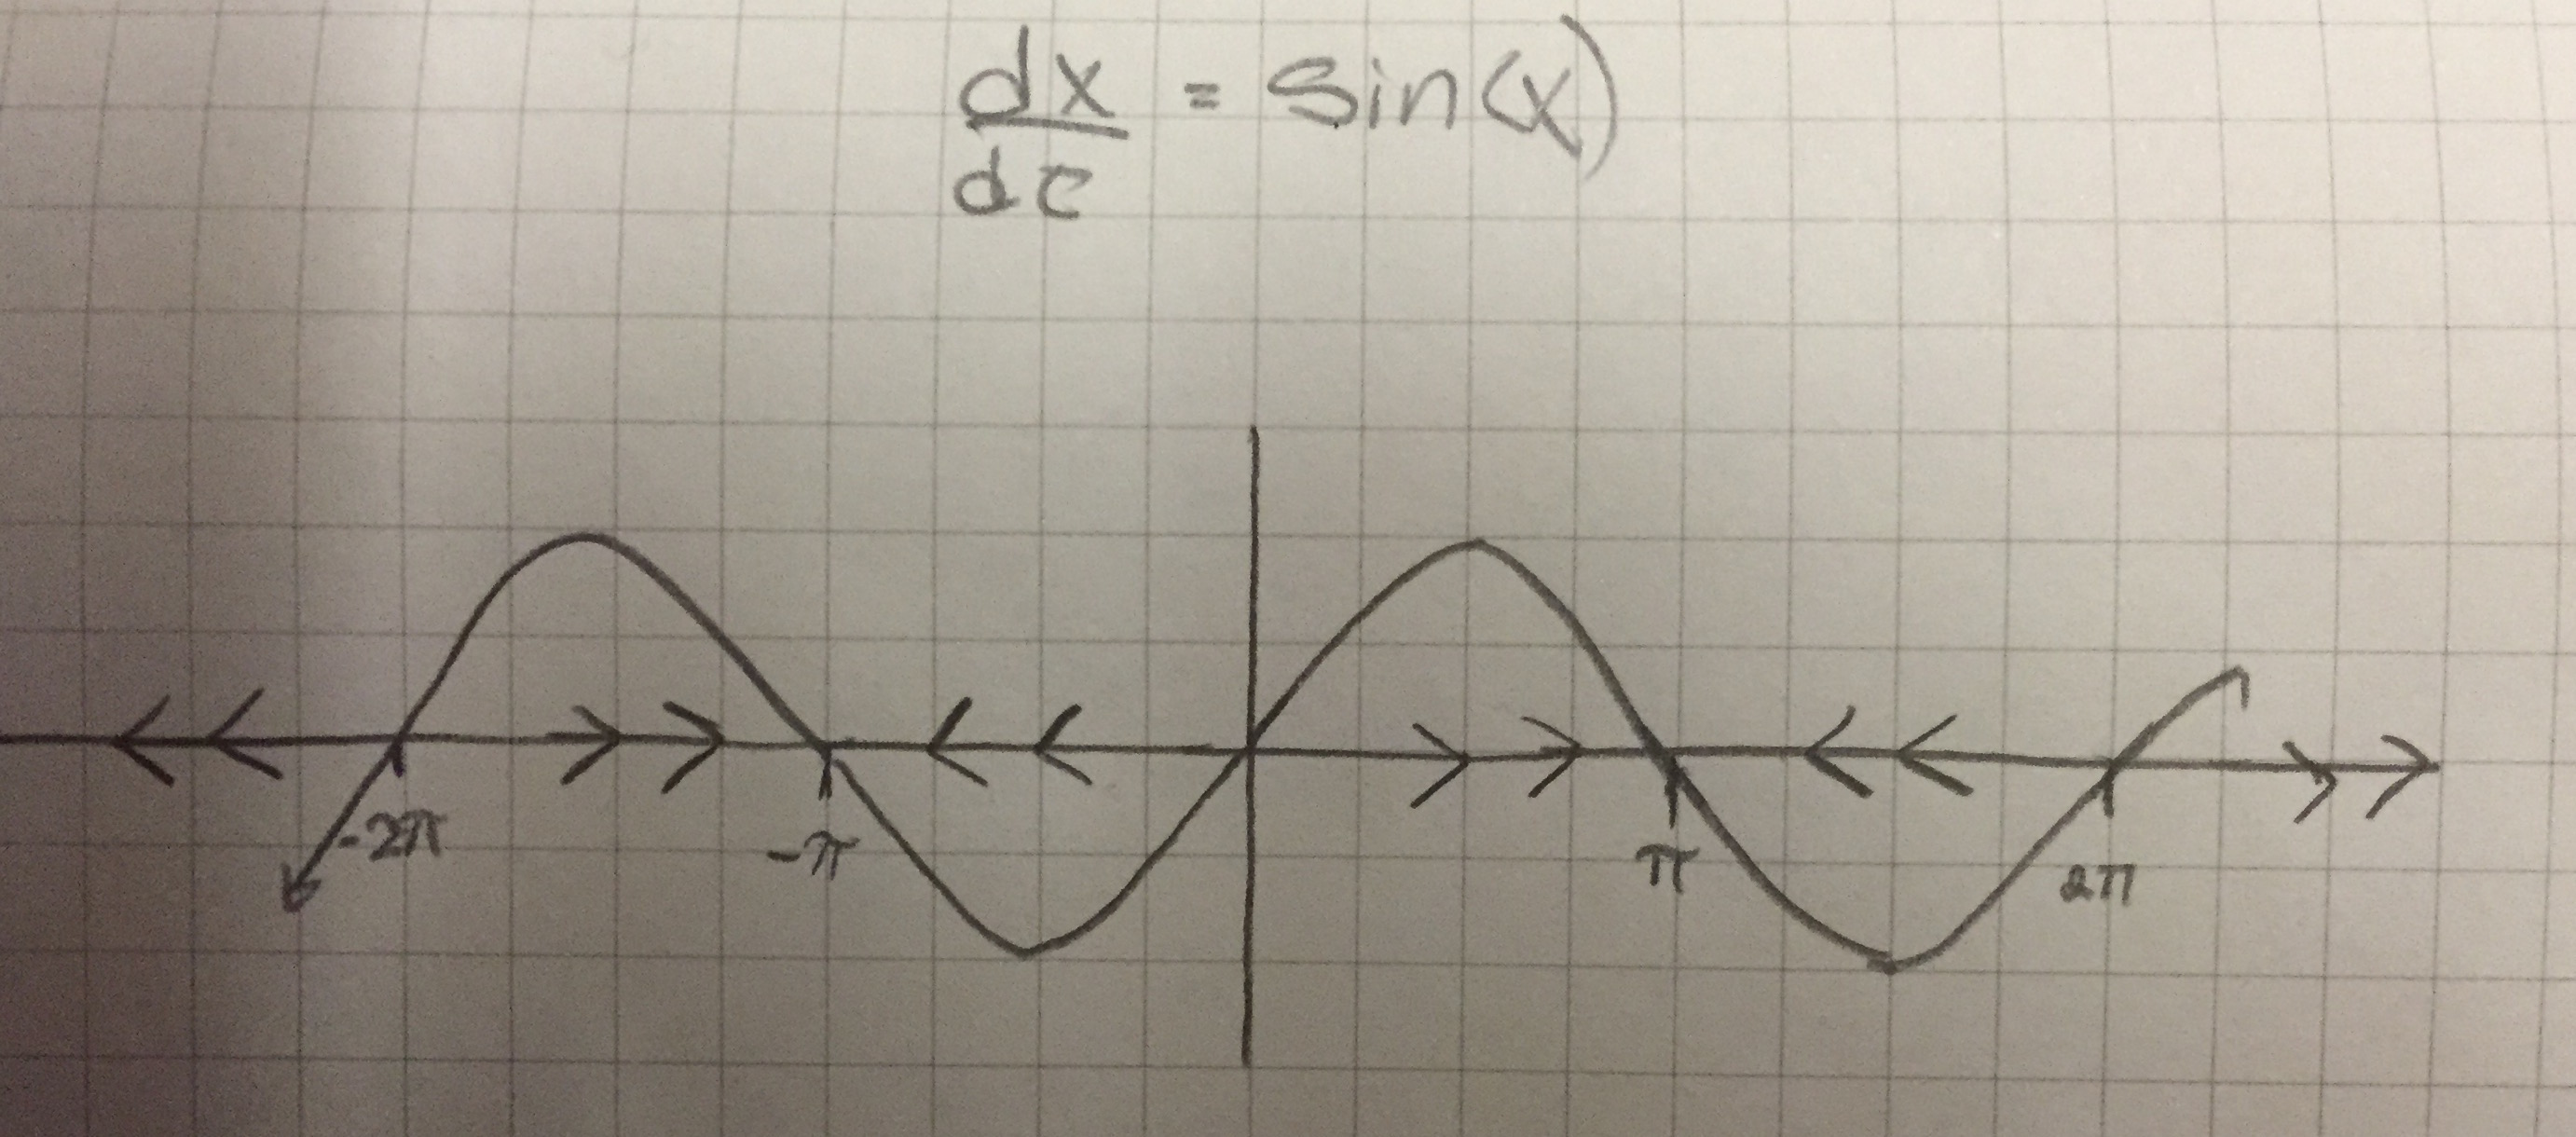
\includegraphics[scale=.05]{phaseportrait2} &
	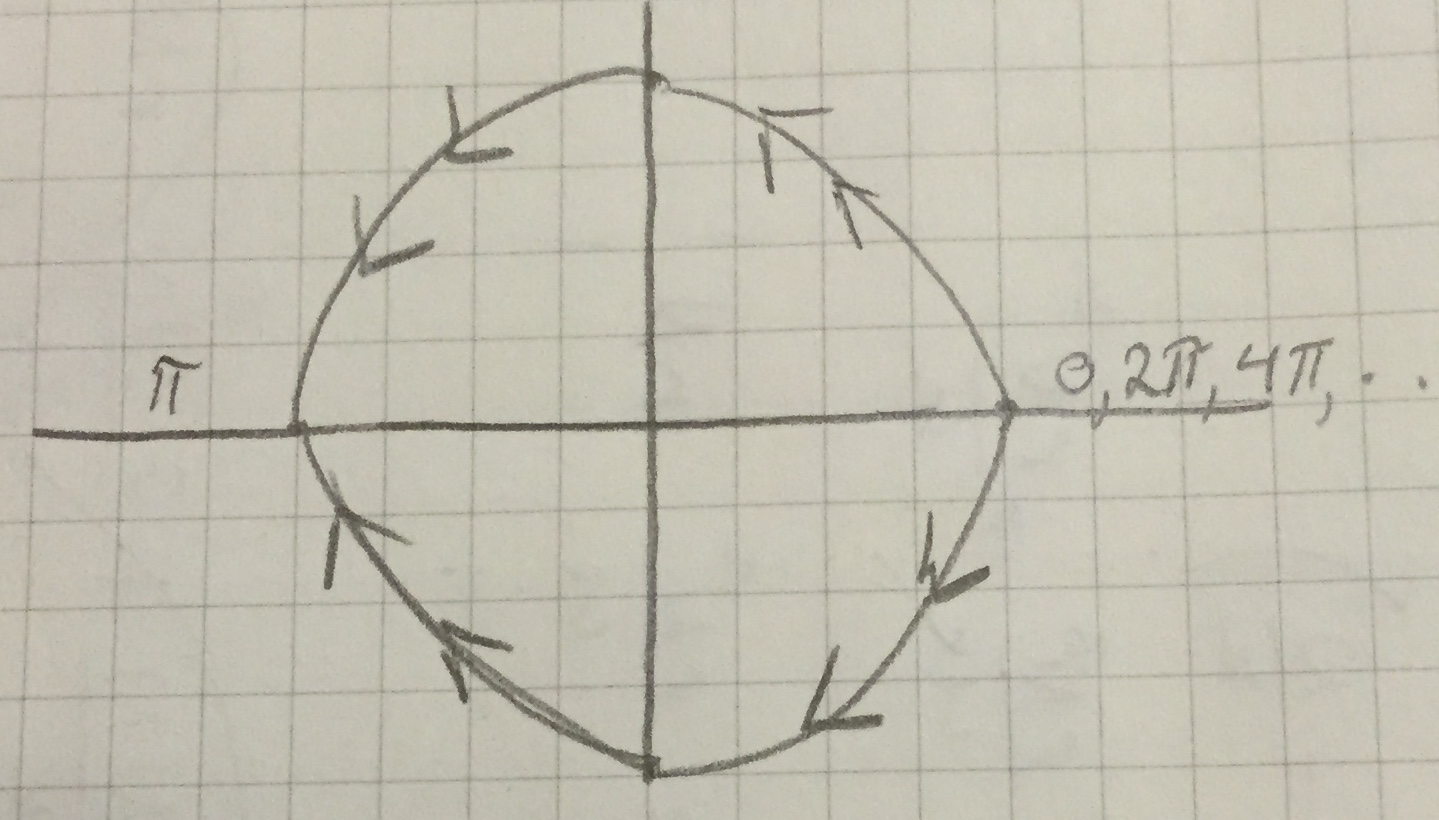
\includegraphics[scale=.07]{phaseportrait2b}
	\end{tabular}
\end{enumerate}	
\end{exercise}

\begin{exercise}{3}
A model for the population growth is given by 
$$\frac{dN}{dt} = f(N) = rN \bigg( \frac{N}{U} - 1 \bigg)\bigg( 1 - \frac{N}{K} \bigg), \qquad N(0) = N_0$$
where $r, K, U$ are positive parameters with $U < K$.

\begin{enumerate}
\item[a)] Sketch the function $f(N)$ and find the equilibrium solution.
\item[b)] Find the linear stability of each equilibrium solution.
\item[c)] Draw the phase portrait and sketch some of the solutions for different $N_0$ (do not solve the ODE).
\item[d)] Discuss the behavior of $N(t)$ as $t \rightarrow \infty$.
\item[e)] Discuss the behavior of $N(t)$ for small $N_0$. This is called critical depensation.
\end{enumerate}

\textbf{Solution}
\\
\begin{enumerate}
	\item[a)] The function is sketched below. The equilibrium solutions are $N = 0, N = K$, and $N = U$. \\
	\begin{center}
		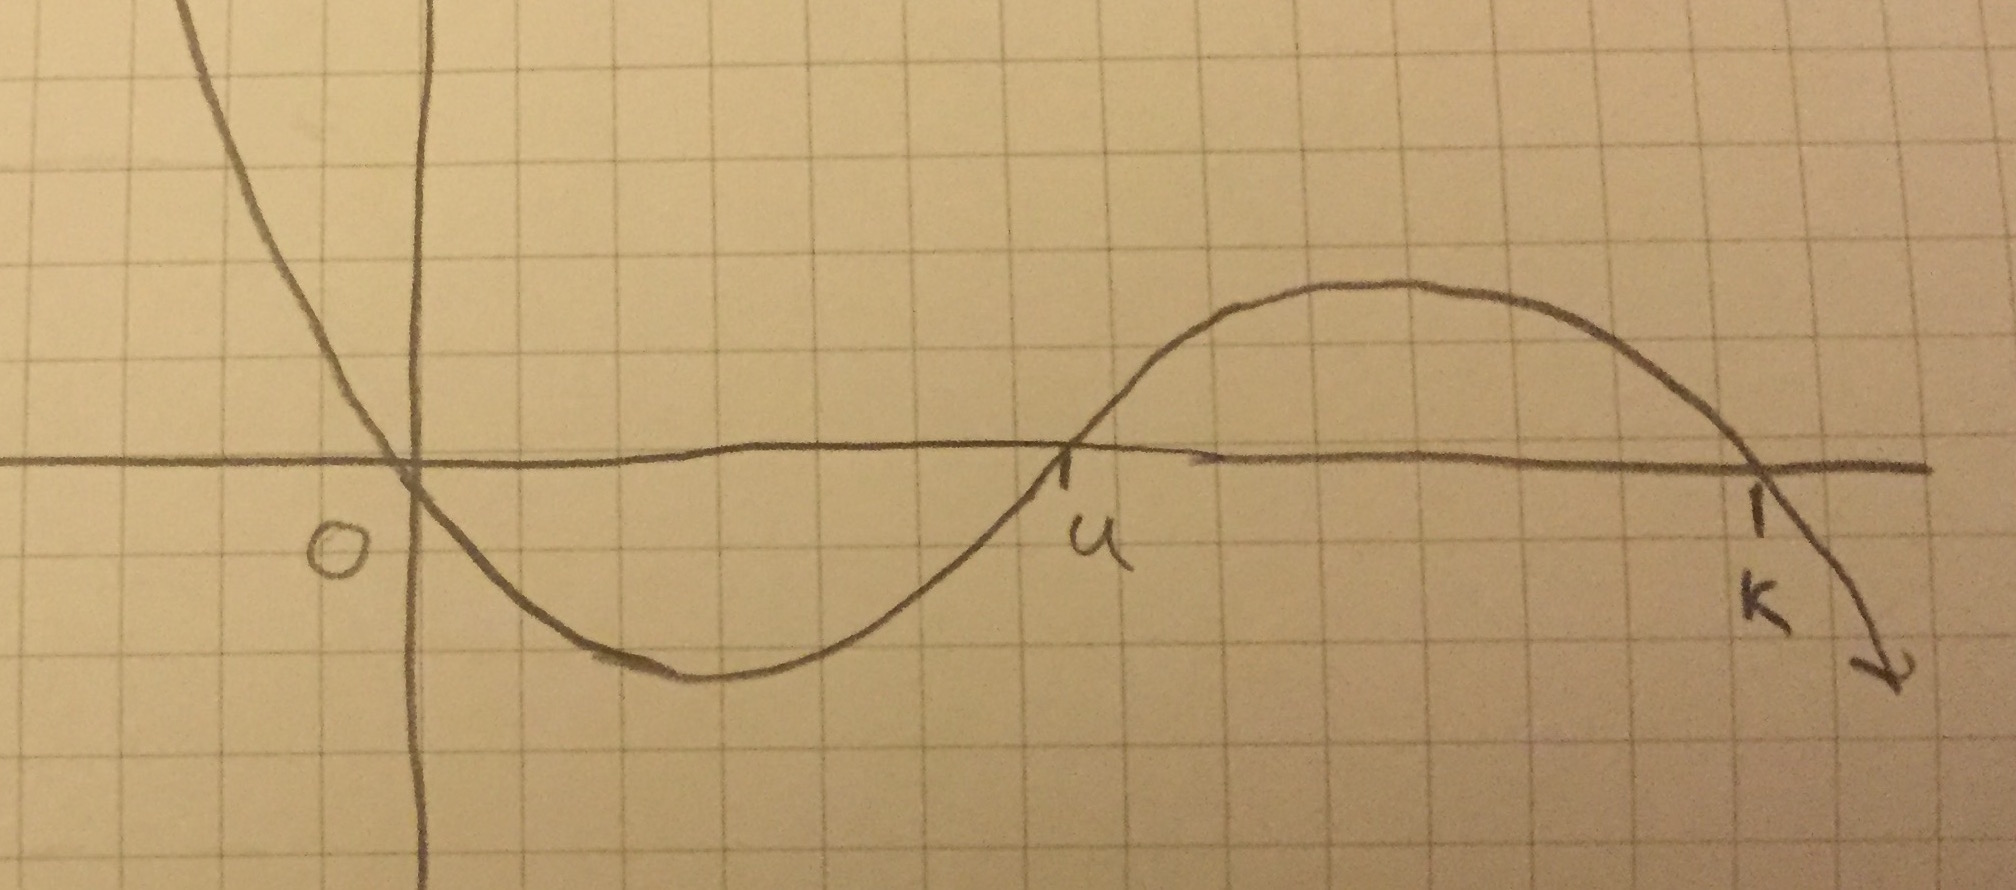
\includegraphics[scale=.06]{graph}
	\end{center}
	\item[b)] The equilibrium solutions $N = 0, N = K$ are both stable solutions. The solution $N = U$ is unstable. 
	\item[c)] The following pictures represents the phase diagram: \\
	\begin{center}
	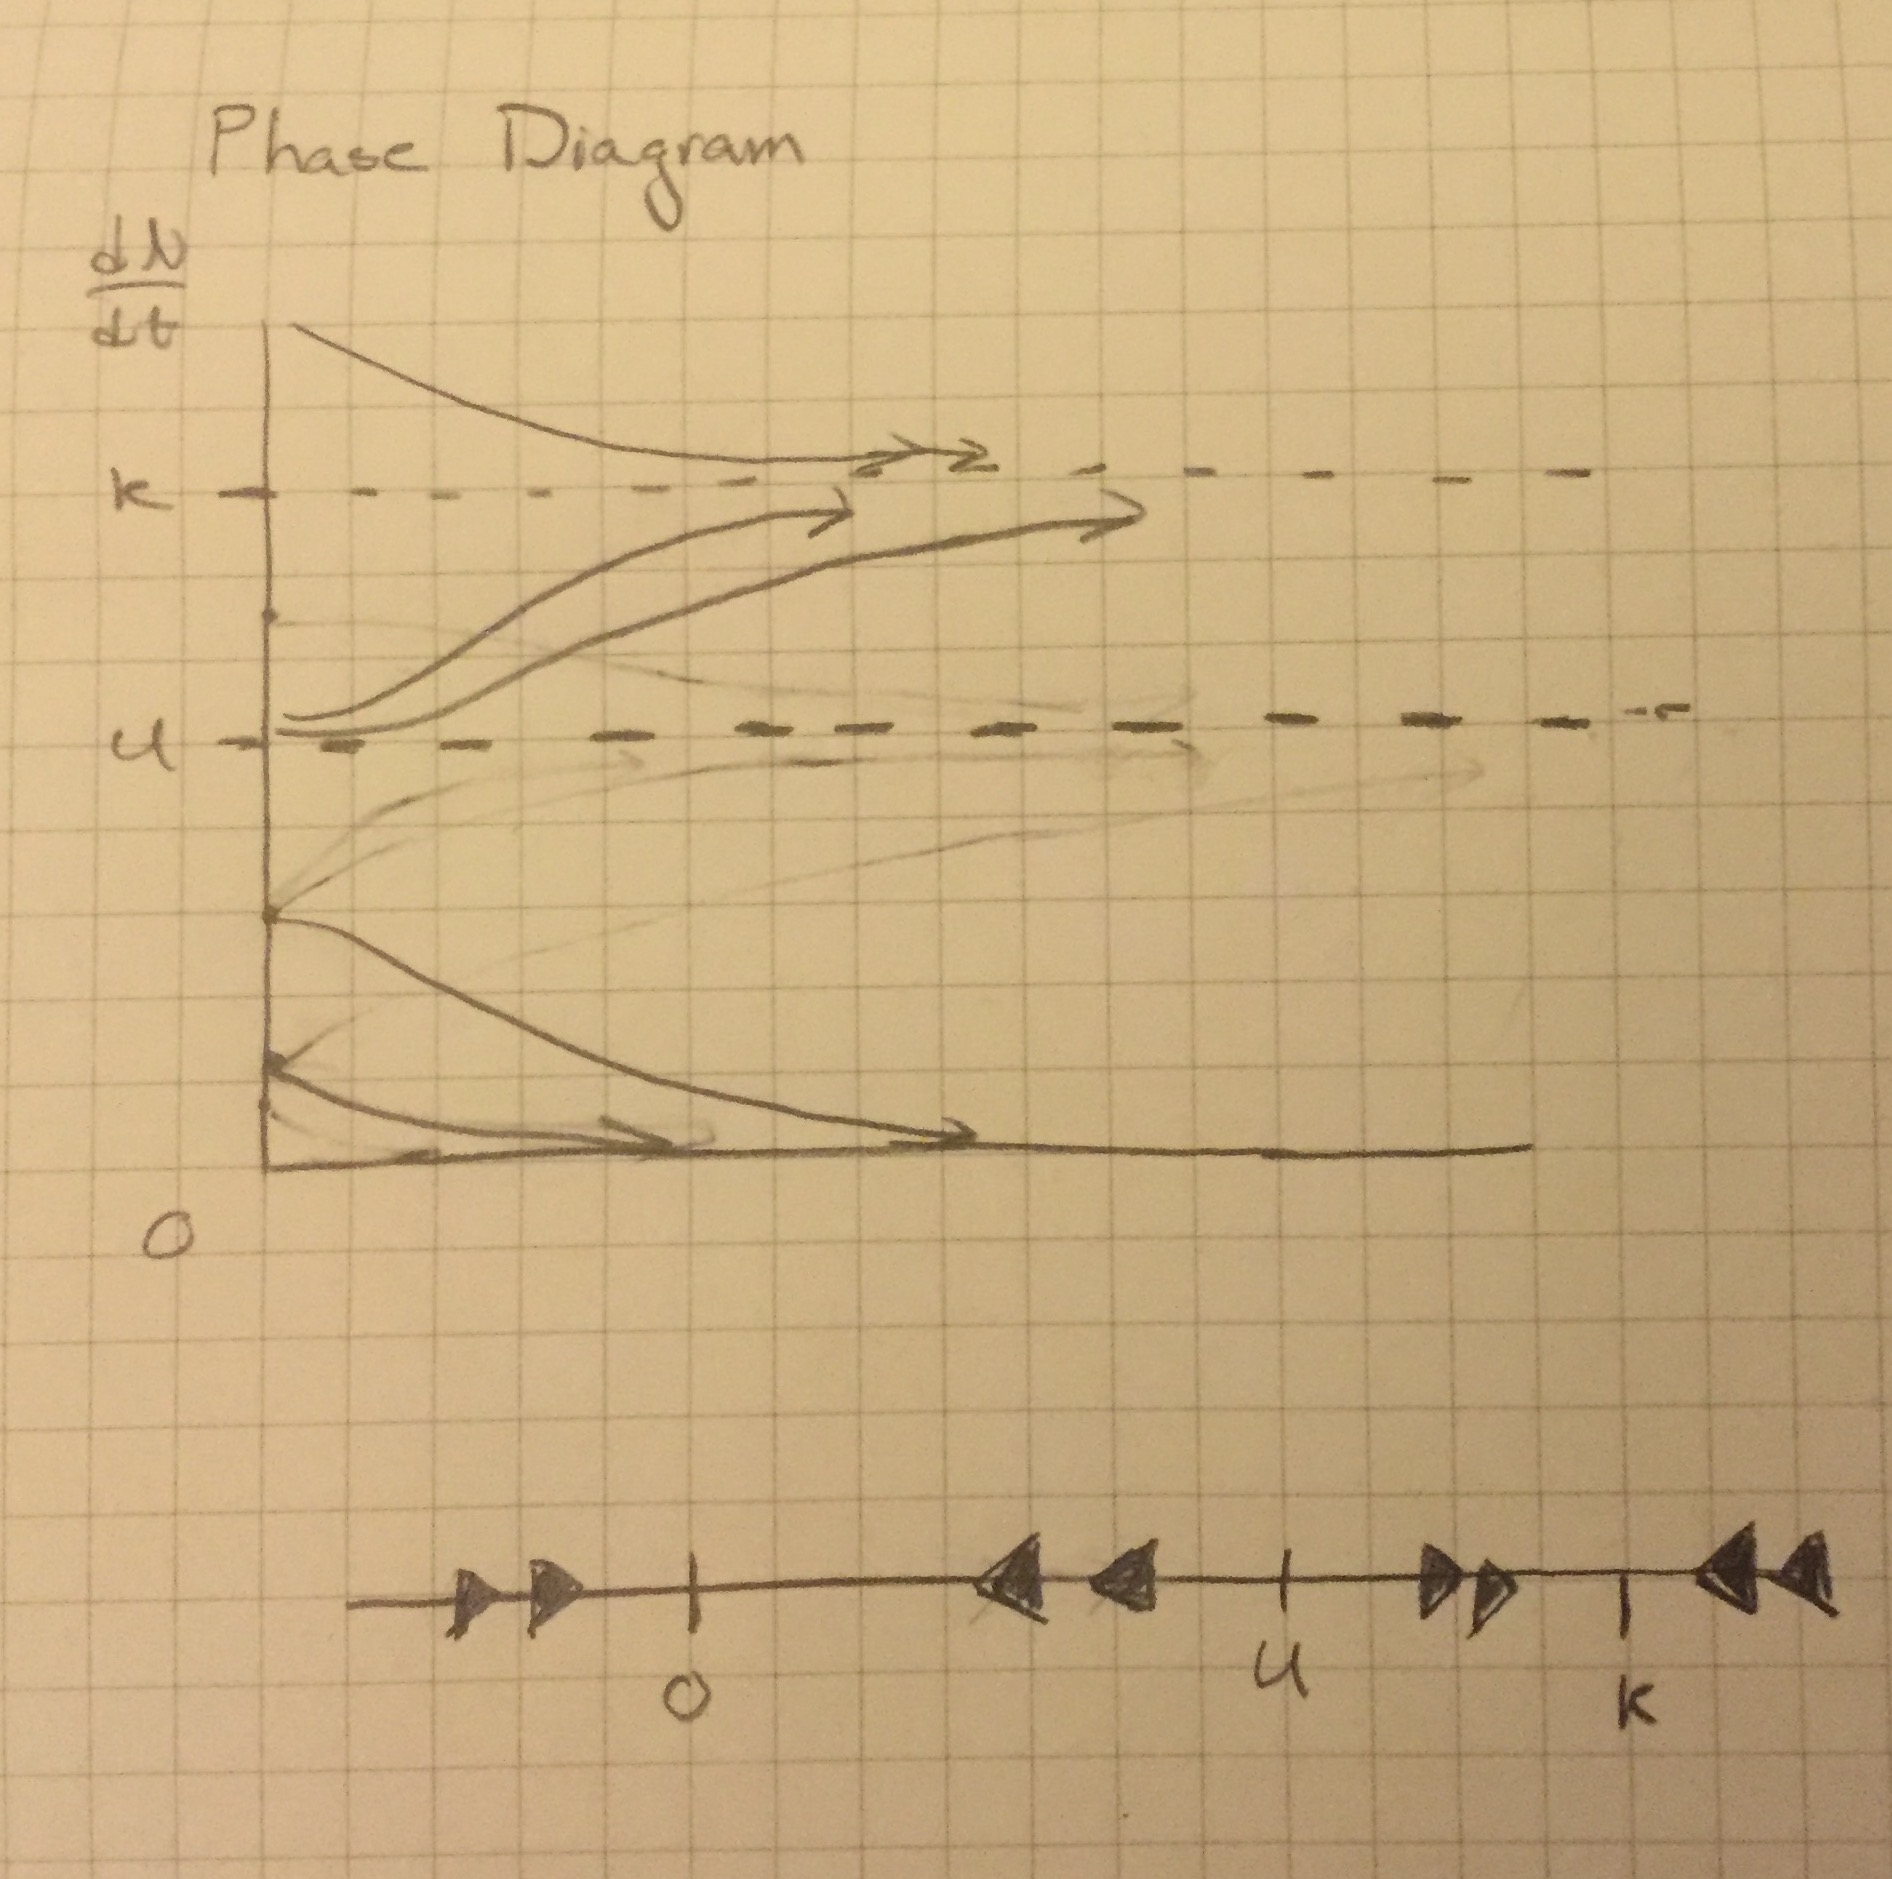
\includegraphics[scale=.08]{phasediagram3}
	\end{center}
	\item[d)] As $t \rightarrow \infty$, $N(t)$ approaches one of the equilibrium solutions. Which solution it approaches is dependent on the initial starting value. If $N < U$ then $N(t) \rightarrow 0$. If $N > U$, then $N(t) \rightarrow K$. 
	\item[e)] For starting values close to $0$ we see that the solution very quickly approaches $0$. This is called depensation, as noted in the problem statement above. Essentially this indicates a point in the population at which a reduced proportion of offspring survive to maturity. 
\end{enumerate}
\end{exercise}

% --------------------------------------------------------------
%     You don't have to mess with anything below this line.
% --------------------------------------------------------------
 
\end{document}